\subsection{Seriel kommunikation}

\subsubsection{Implementering af SPI}
SPI forbindelsen blev mellem de to enheder blev etableret med 6 ledninger som set på figur xx. En til MOSI, MISO, CLK, SS, VCC og GND (reference til SPI).
Udgangen for DevKit8000 er valgt på baggrund af datasheet for denne enhed (reference til devkit datasheet). GPIO pins på PSoC er valgfrie, og konfigureres 
i PSoC-creator til de ønskede værdier.

\begin{figure}[H]
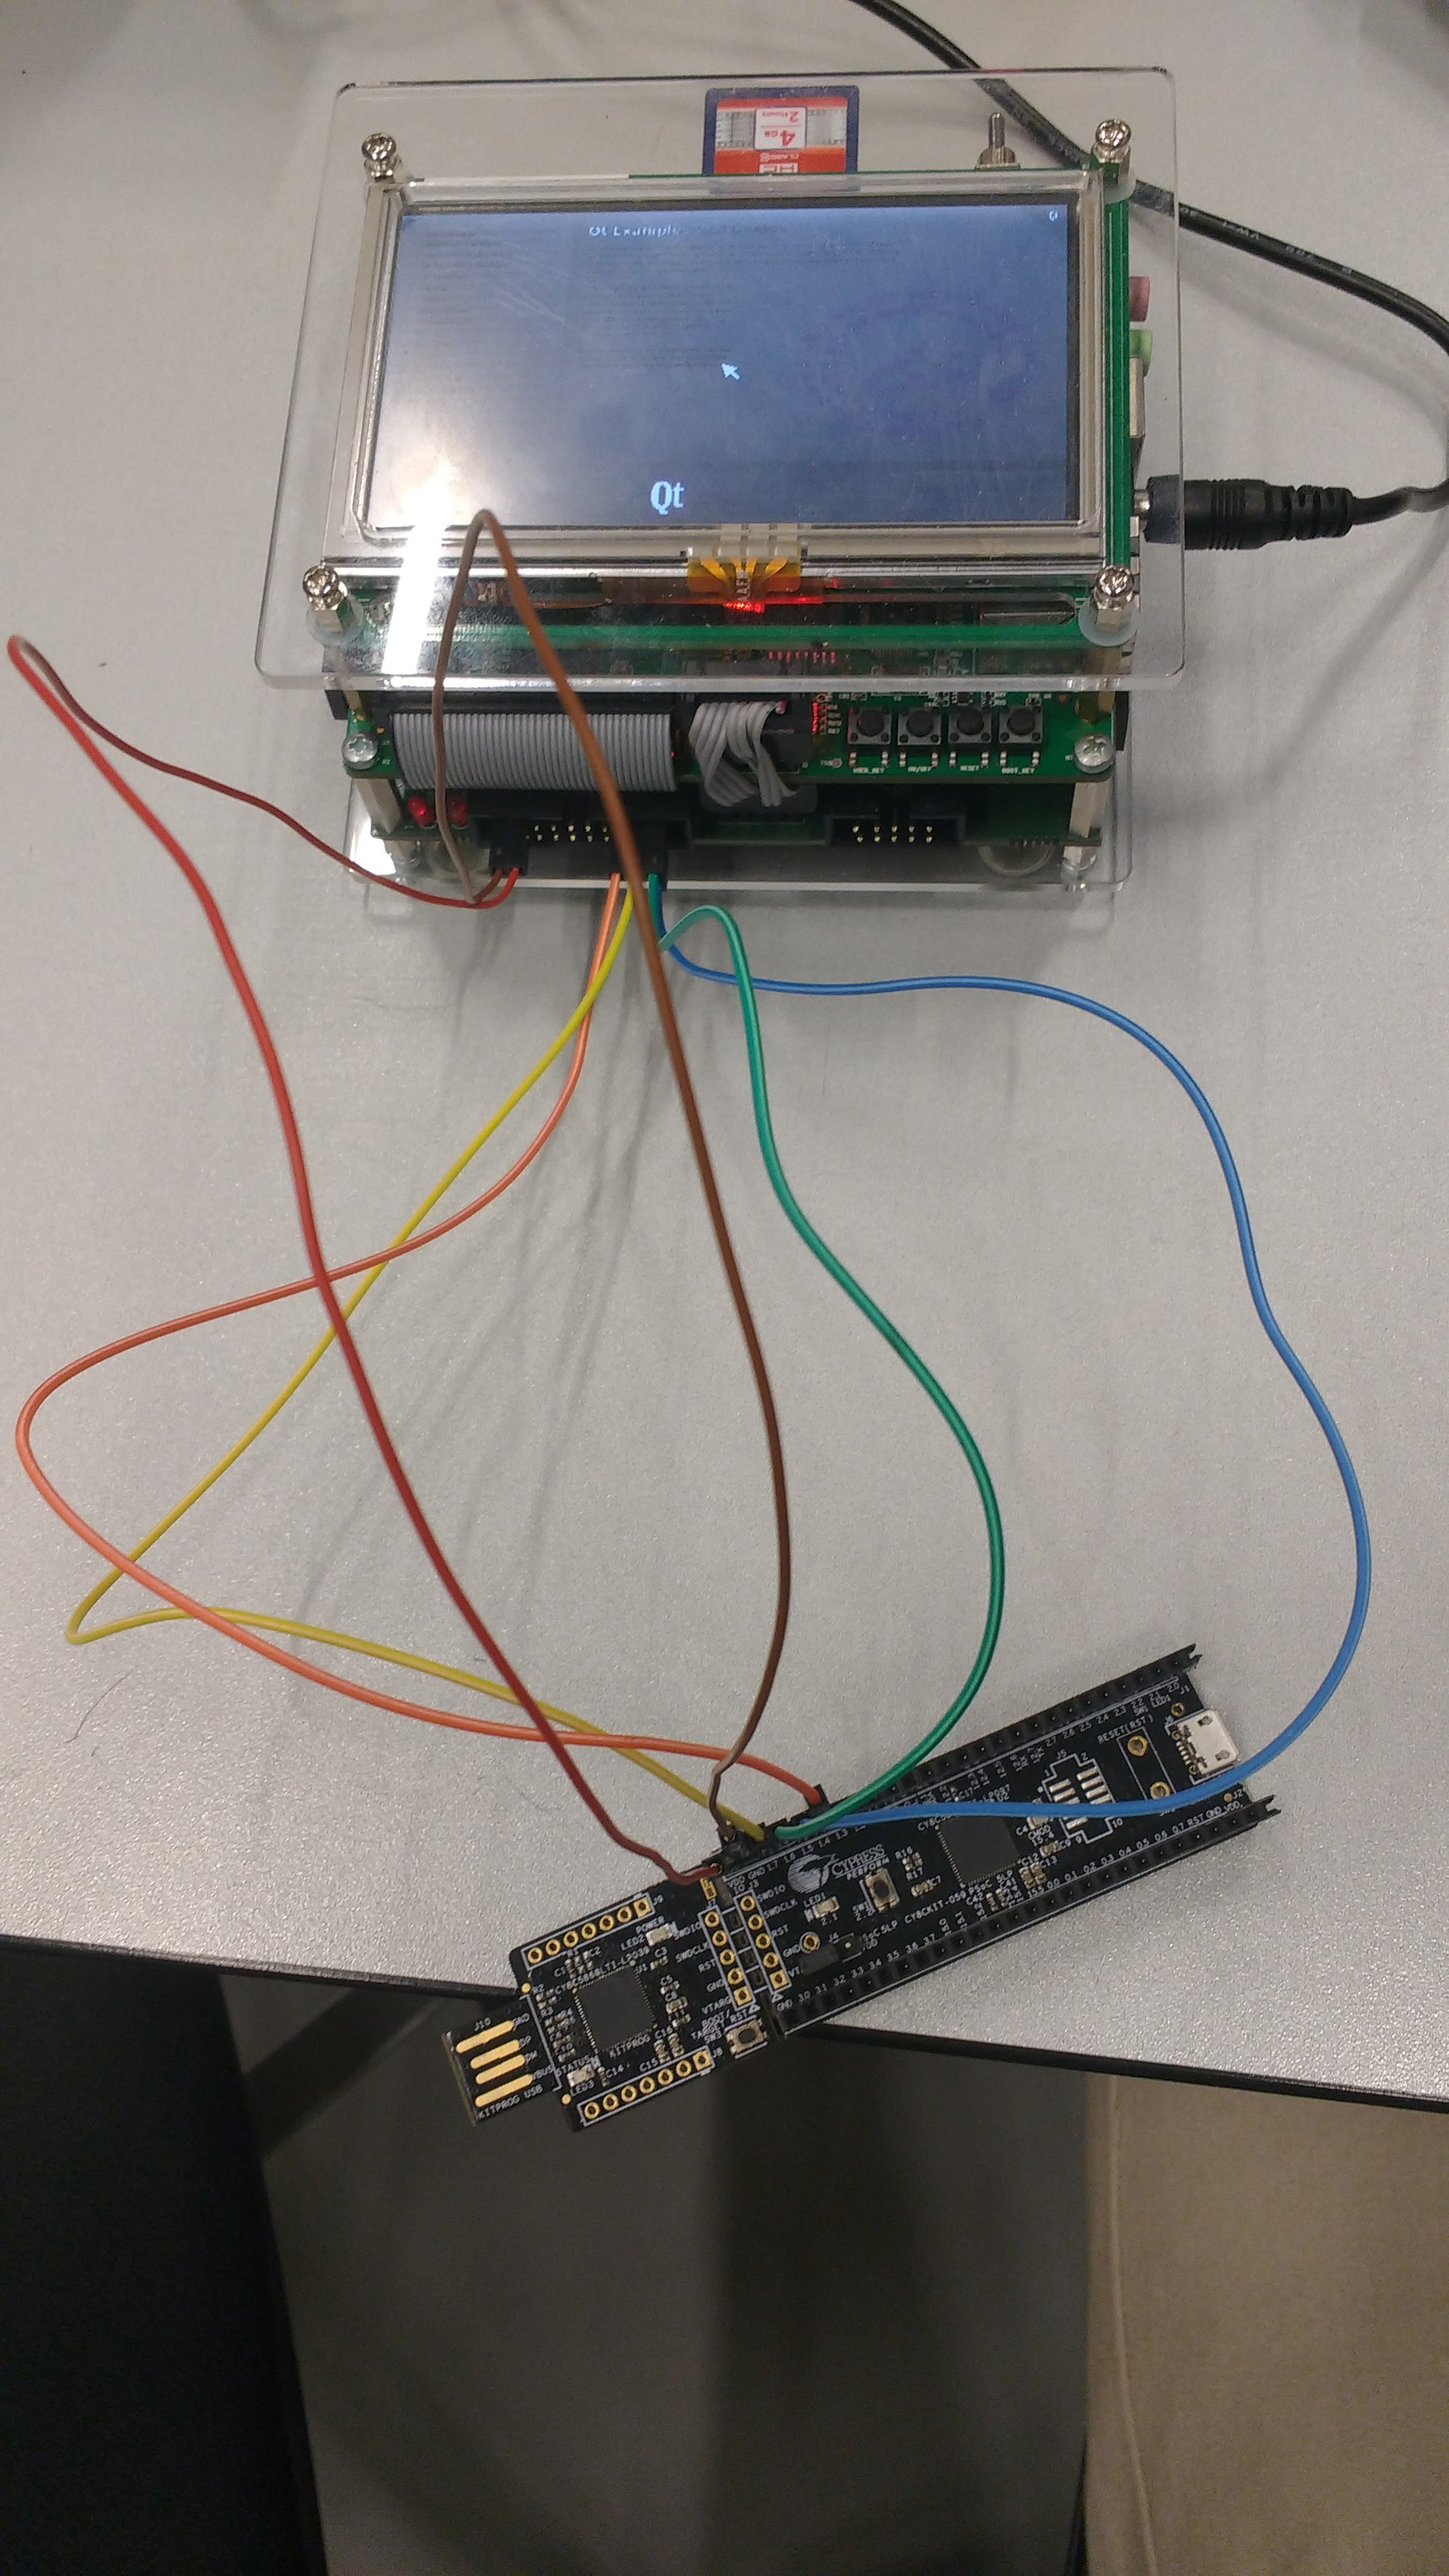
\includegraphics[scale=0.6]{tex/TeImRe/SPI/Realisering_devkit_psoc}
\caption{Den fysiske forbindelese mellem Devkit800 og PSoC Master}
\end{figure}

Som nævnt i Design afsnittet for SPI (reference til design), har der ikke været adgang til koden for SPI device driveren på DevKit8000, hvorfor implementeringen
af denne ikke kan beskrives nærmere. \\

Til implementeringen af SPI på PSoC Master og PSoC Slave er der benyttet PSoC creator, som med et drag-and-drop interface gør det nemt at opsætte SPI forbindelsen. 
Derudover indeholder programmet en main fil hvori der er implementeret en håndtering af de modtagende databits. Koden består dybest set at en interrupt service 
rutine (ISR), som kaldes hver gang, der er blevet læst en data-byte ind på Rx-bufferen. Den tilhørende interrupt-rutine vil fungere som en state-machine, 
hvor den pågældende data-byte læses i en switch, som, alt efter kommandoen, sætter en variabel, der læses i PSoC'ens tilhørende \textit{main}-funktion, til en 
bestemt værdi. I \textit{main}-funktionen skal der da påkaldes de relevante metoder, som skal følge den modtagne kommando. Grunden til denne implementering er, 
at holde så meget af programmets funktionalitet så opdelt som muligt for at opretholde princippet om høj samhørighed - lav kobling. For mere information omkring 
koden for PSoC master og PSoC Slave henvises til bilag(navn på bilag).   


\subsubsection{Test af SPI}

\textbf{DevKit8000-PSoC Master:}\\
Til test af denne forbindelsen blev der sendt data fra DevKit8000, ved at skrive ud til den fil i /dev som var forbundet til SPI hardwaren. Herefter blev der
med Logic analyser målt MOSI (udgangen på DevKit8000), CLK(klokken), SS(slave select). Der blev kigget på om de rigtige databits blev skrevet ud
til MOSI, om SS gik lav ved dataoverførelse, og om CLK havde den rigtige clockmode. Efterfølgende blev der også læst fra den samme fil i /dev, og der blev målt
på MISO(Indgangen på DevKit8000).\\


\textbf{PSoC Master - PSoC Slave:} \\
Til test af PSoC-PSoC forbindelsen, blev der tilføjet et UART modul i PSoC creator. Dette gjorde det muligt at skrive de resultater som blev send til PSoC 
enhederne til en terminal på en PC, hvor disse nemt kunne aflæses. Der blev også målt med Logic Analyzer for at teste om de fire forbindelser MISO, MOSI, CLK 
og SS og rigtig ud ligsom i testen mellem DevKit8000 og PSoC Master. På figur xx ses testopstilling for PSoC-PSoC\\

\begin{figure}[H]
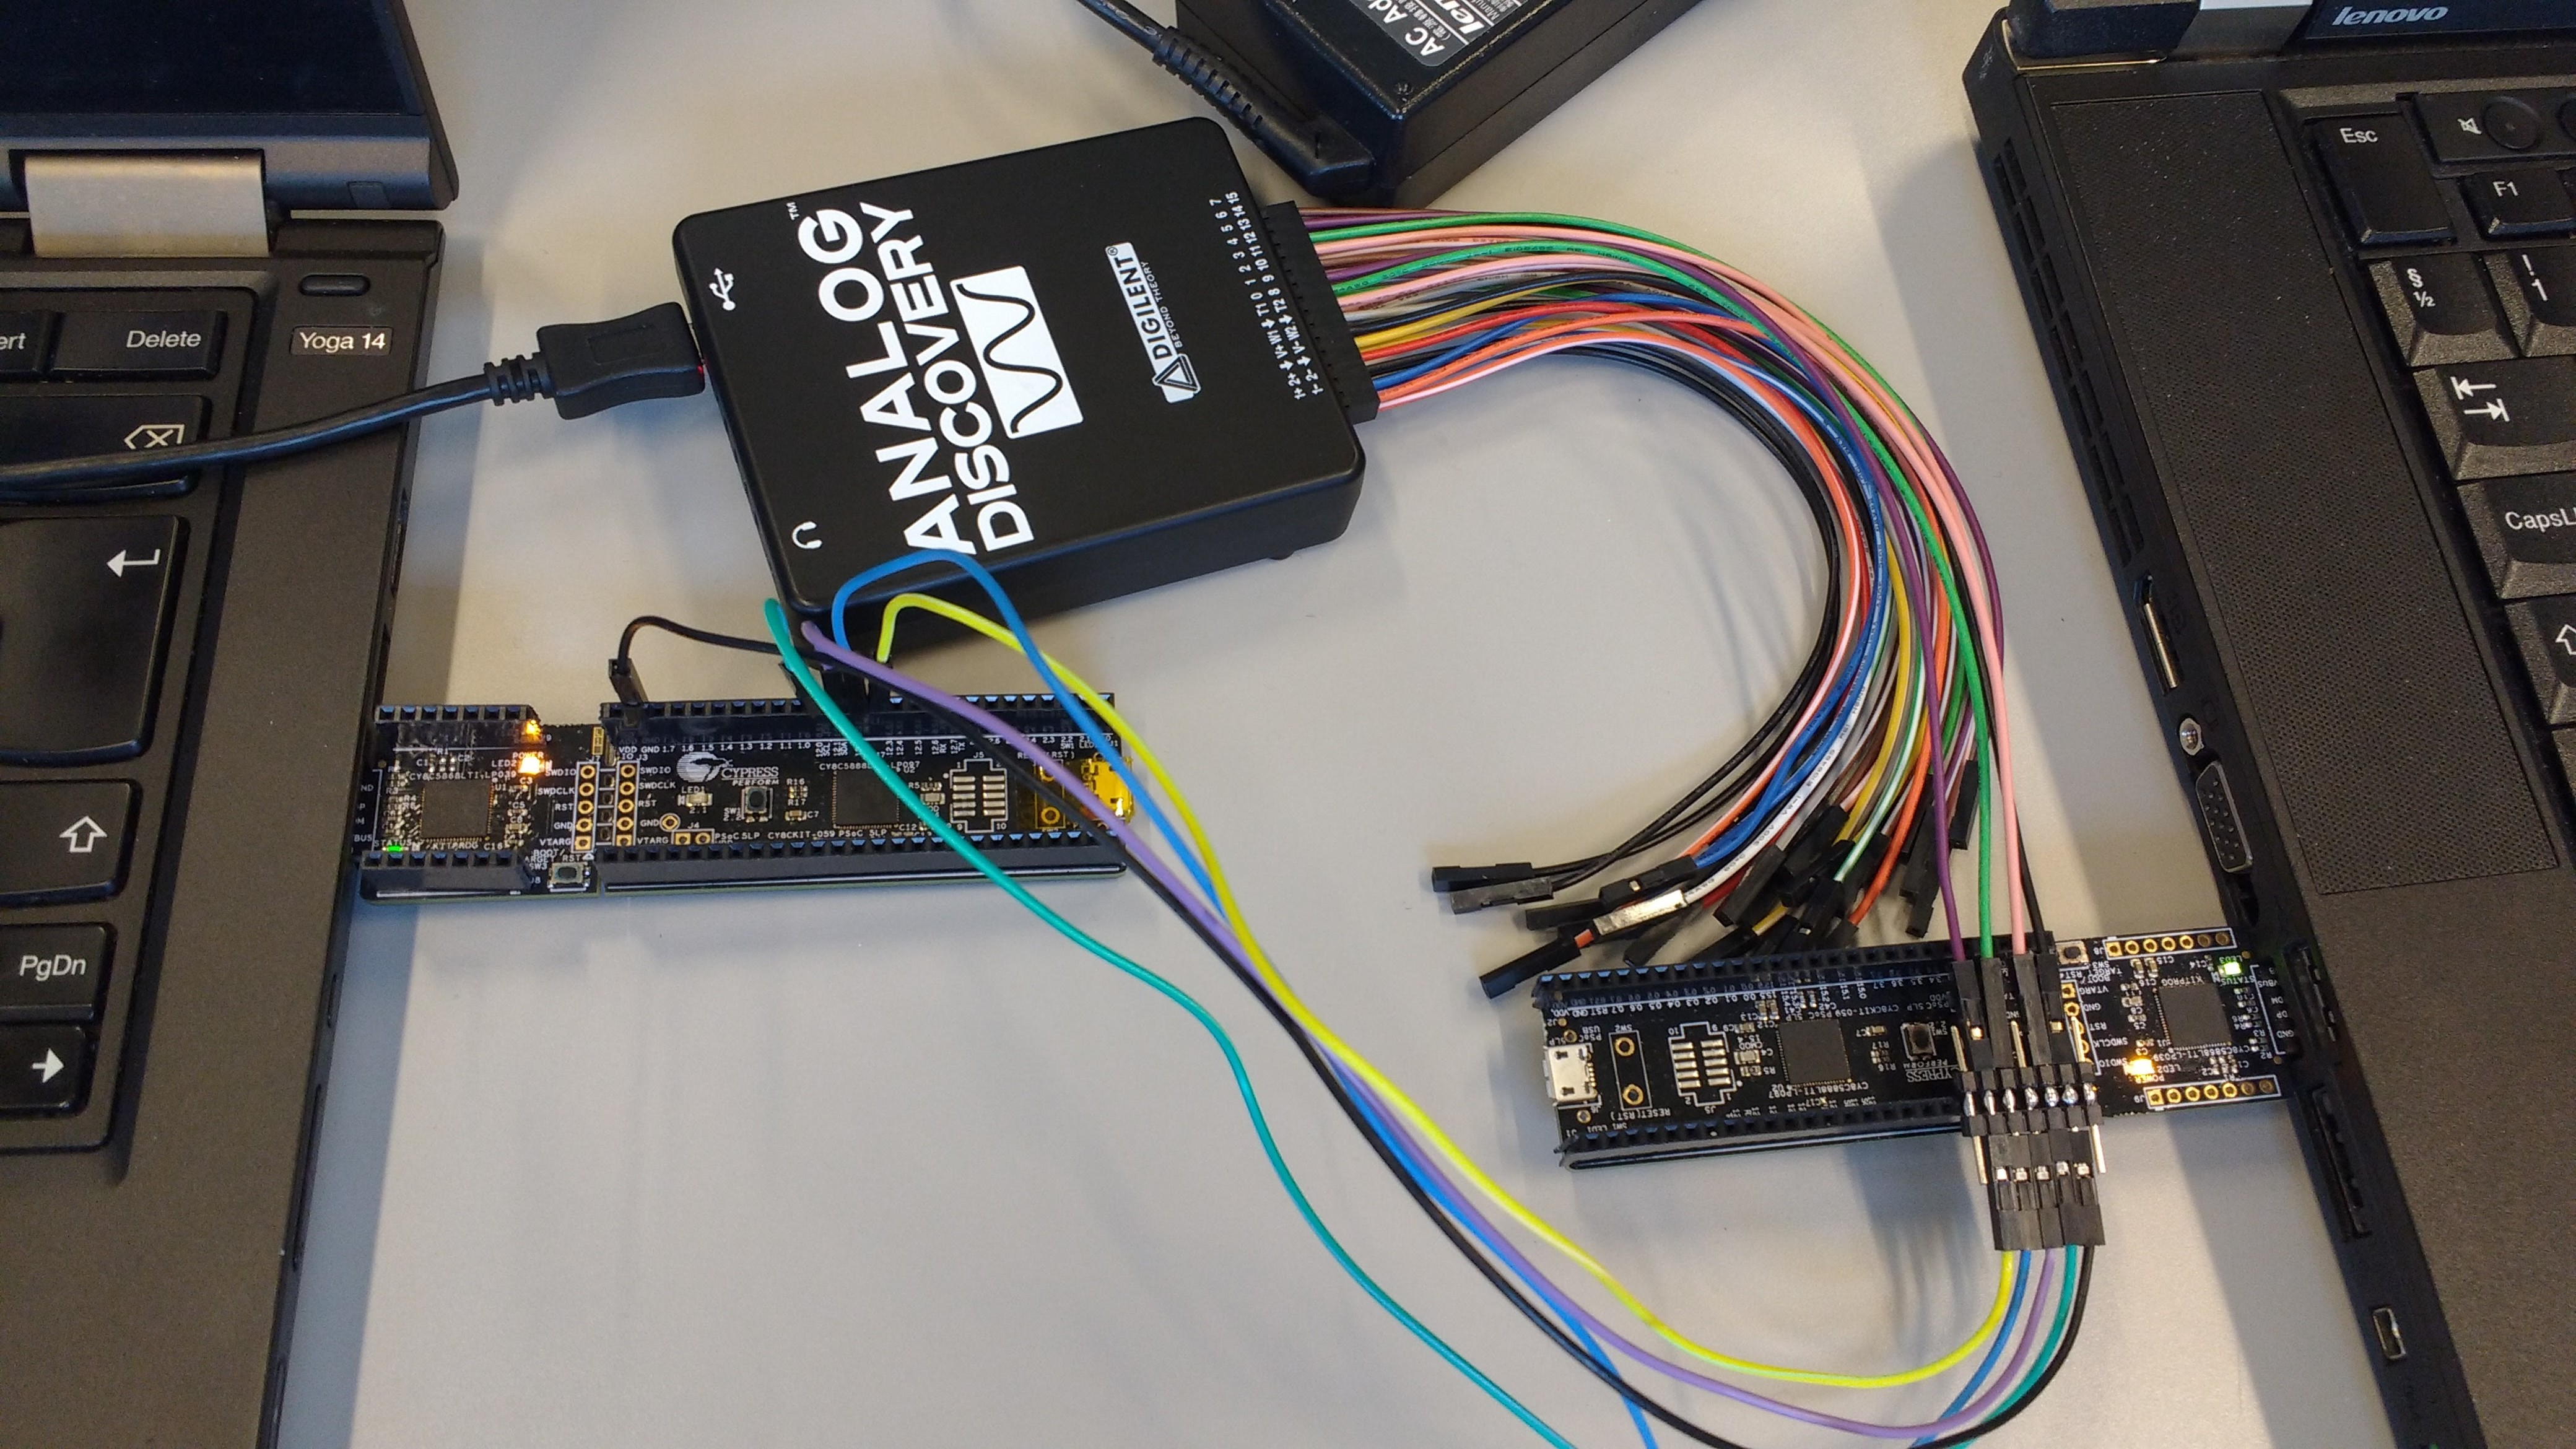
\includegraphics[scale=0.6]{tex/TeImRe/SPI/SPI_testAnalog}
\caption{testopstilling for PSoC Master/PSoC Slave forbindelsen}
\end{figure}

\subsection{Resultater for SPI kommunikation}
\textbf{DevKit8000-PSoC Master:}\\
På figur xx ses resulater på Logic Analyzer når der skrives til PSoC master fra terminalen på Devkit8000.

\begin{figure}[H]
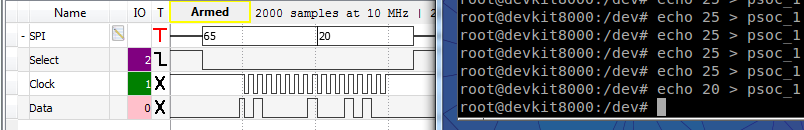
\includegraphics[scale=0.6]{tex/TeImRe/SPI/Analog_devkit_echo_psoc_1}
\caption{Udskrift fra Logic Analyzer fra test af SPI forbindelse mellem Devkit og PSoC Master}
\end{figure}

Resultater for læsningen af PSoC Master gav kun succesfuldt resultater ved en enkelt test. Derudover kunne der ikke læses fra PSoC master
Hvilket betyder at der ikke er dokumentet en succesfuld aflæsning af MISO forbindelsen. Selv efter mange forsøg, og med hjælp fra undervisere i HAL, blev 
dette problem aldrig løst.

\textbf{PSoC Master - PSoC Slave:} \\
På figur xx ses udskrift Logic Analyzer og PC Terminal. Der er i denne test blevet skrevet værdien 5 til PSoC slave. Billeder for test af MISO er udeladt, men
gav dog samme resultat.

\begin{figure}[H]
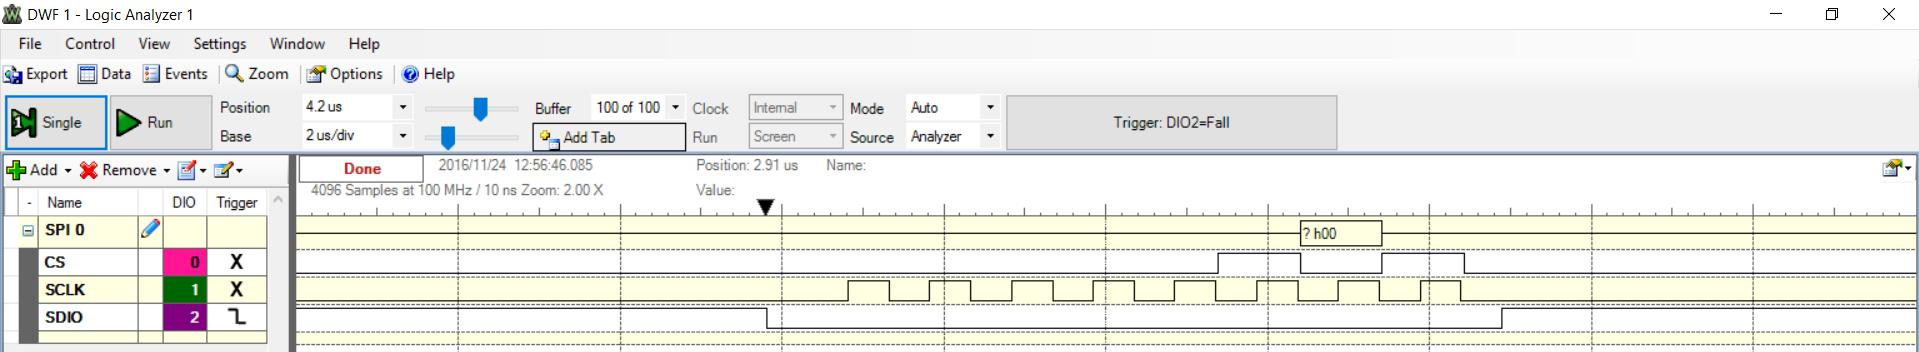
\includegraphics[scale=0.6]{tex/TeImRe/SPI/Logic_analyzer}
\caption{Udskrift fra Logic Analyzer fra test af SPI forbindelse mellem PSoC Slave og PSoC Master}
\end{figure}

\begin{figure}[H]
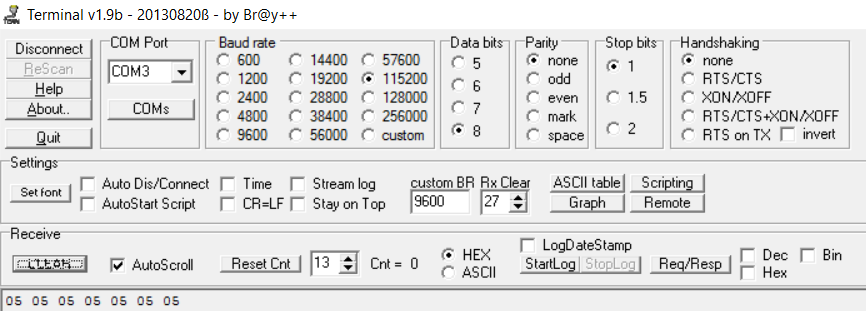
\includegraphics[scale=0.6]{tex/TeImRe/SPI/Terminal_spi_slave}
\caption{Udskrift fra terminal fra test af SPI forbindelse mellem PSoC Slave og PSoC Master}
\end{figure}

\subsection{Diskussion af resultater for SPI kommunikation}
textbf{DevKit8000-PSoC Master:}\\
Som det ses på figur xx, blev der succesfuldt sendt de korrekte databits ud på SPI MOSI, SS gik også lav ved dataoverførelse hvilket er meget vigtigt
for at sikre, at den korrekte slave i vores tilfælde "PSoC Master" modtager kommandoerne. CLK ser rigtig ud med den clock mode som er specificeret.
Dette ses ved at CLK starter høj og skifter bits på nedafgående flanke, og læser på opadgående flanke. Dette svarer til CPHA = 1 og CPOL = 1, hvilket også var 
den opsæninger der er lavet for denne SPI forbindelse.\\

Problemet med MISO forbindelsen betød at projektets prototype ikke kunne sende status beskeder til brugeren, hvilket naturligvis var en stor skuffelse for
gruppen. Problemet ligger højst sandsynlig på selve PSoC, da der ikke læses noget data på MISO forbindelsen, og det derfor ikke har noget med DevKit8000 af gøre.


\textbf{PSoC Master - PSoC Slave:} 
Her ses igen er det er de rigtige databits som bliver sendt, og SS går ligeleder lav som den burde. Det ser dog ud til at clock mode ikke helt passer med
CPHA = 0 og CPOL = 0, som den var sat til. CLK starter lav som den skal, men ser ud til at skrifte på nedadgående flanke og læse på opadgående. Dette
er ikke korrekt, og grunden hertil er uvis. Men som det ses på figur xx, så udskrives de korrekte bits til terminalen på PC, hvilket må betyde at 
PSoC Slave modtager de korrekte bits, og derfor burde denne forbindelse virke fint.\\ 

